\documentclass{beamer}
\usepackage[utf8]{inputenc}
\usepackage{lmodern}
\usepackage[brazil]{babel}
\usetheme{Madrid}

% -------------------------------------------------
% Identidade Visual - Centro Paula Souza
% -------------------------------------------------
\definecolor{cpsred}{RGB}{153,0,0}      % Vermelho institucional
\definecolor{cpsgray}{RGB}{85,85,85}    % Cinza técnico

\usecolortheme[named=cpsred]{structure}
\setbeamercolor{title}{fg=white,bg=cpsred}
\setbeamercolor{frametitle}{fg=white,bg=cpsred}
\setbeamercolor{structure}{fg=cpsred}
\setbeamercolor{normal text}{fg=black,bg=white}
\setbeamercolor{itemize item}{fg=cpsred}

\usepackage{ragged2e}
\usepackage{hyperref}

\setbeamertemplate{headline}{} 

% -------------------------------------------------
% Rodapé padrão
% -------------------------------------------------
\setbeamertemplate{footline}[frame number]
\addtobeamertemplate{footline}{
  \hfill\usebeamercolor[fg]{frametitle}{\hspace{-1.5cm}\scriptsize Amanda Oliveira, Arthur Fudali, Diego Souza, Giovana Albanês, Igor Leite}\hspace{1cm}
}{}

% -------------------------------------------------
% Informações principais
% -------------------------------------------------
\title[Teste de Desempenho Contínuo, Orientado por Visão Computacional]{\textbf{Teste de Desempenho Contínuo, Orientado por Visão Computacional}}
\author{Amanda Oliveira, Arthur Fudali, Diego Souza, Giovana Albanês, Igor Leite}
\date{}

% -------------------------------------------------
% Documento
% -------------------------------------------------
\begin{document}

% Capa
\begin{frame}
    \centering
    \vspace{1cm}
    {\color{cpsred}\Huge\textbf{Teste de Desempenho Contínuo, Orientado por Visão Computacional}}\\[0.8cm]
    {\Large Amanda Oliveira, Arthur Fudali, Diego Souza, Giovana Albanês, Igor Leite}\\[0.4cm]
    \textcolor{cpsgray}{Centro Paula Souza}\\[0.2cm]
    \textcolor{cpsgray}{FATEC Registro}
\end{frame}

% Sumário
\begin{frame}{Sumário}
\tableofcontents
\end{frame}

% -------------------------------------------------
% SEÇÕES E SLIDES
% -------------------------------------------------

\section{Pitch}
\begin{frame}{Pitch}
\justifying
Pitch
\end{frame}

\section{Problematização}
\begin{frame}{Problematização}
\justifying
\begin{enumerate}
  \item Diagnóstico tradicional de TDA é subjetivo e inacessível.
  \item Falta de ferramentas tecnológicas acessíveis.
  \item Dificuldade em mensurar o comportamento atencional em tempo real.
  \item Baixo engajamento em processos avaliativos tradicionais.
\end{enumerate}
\end{frame}

\section{Estado da Arte}
\begin{frame}{Estado da Arte}
\justifying

\begin{columns}[T,onlytextwidth]

    \begin{column}{0.48\textwidth}
        \centering
        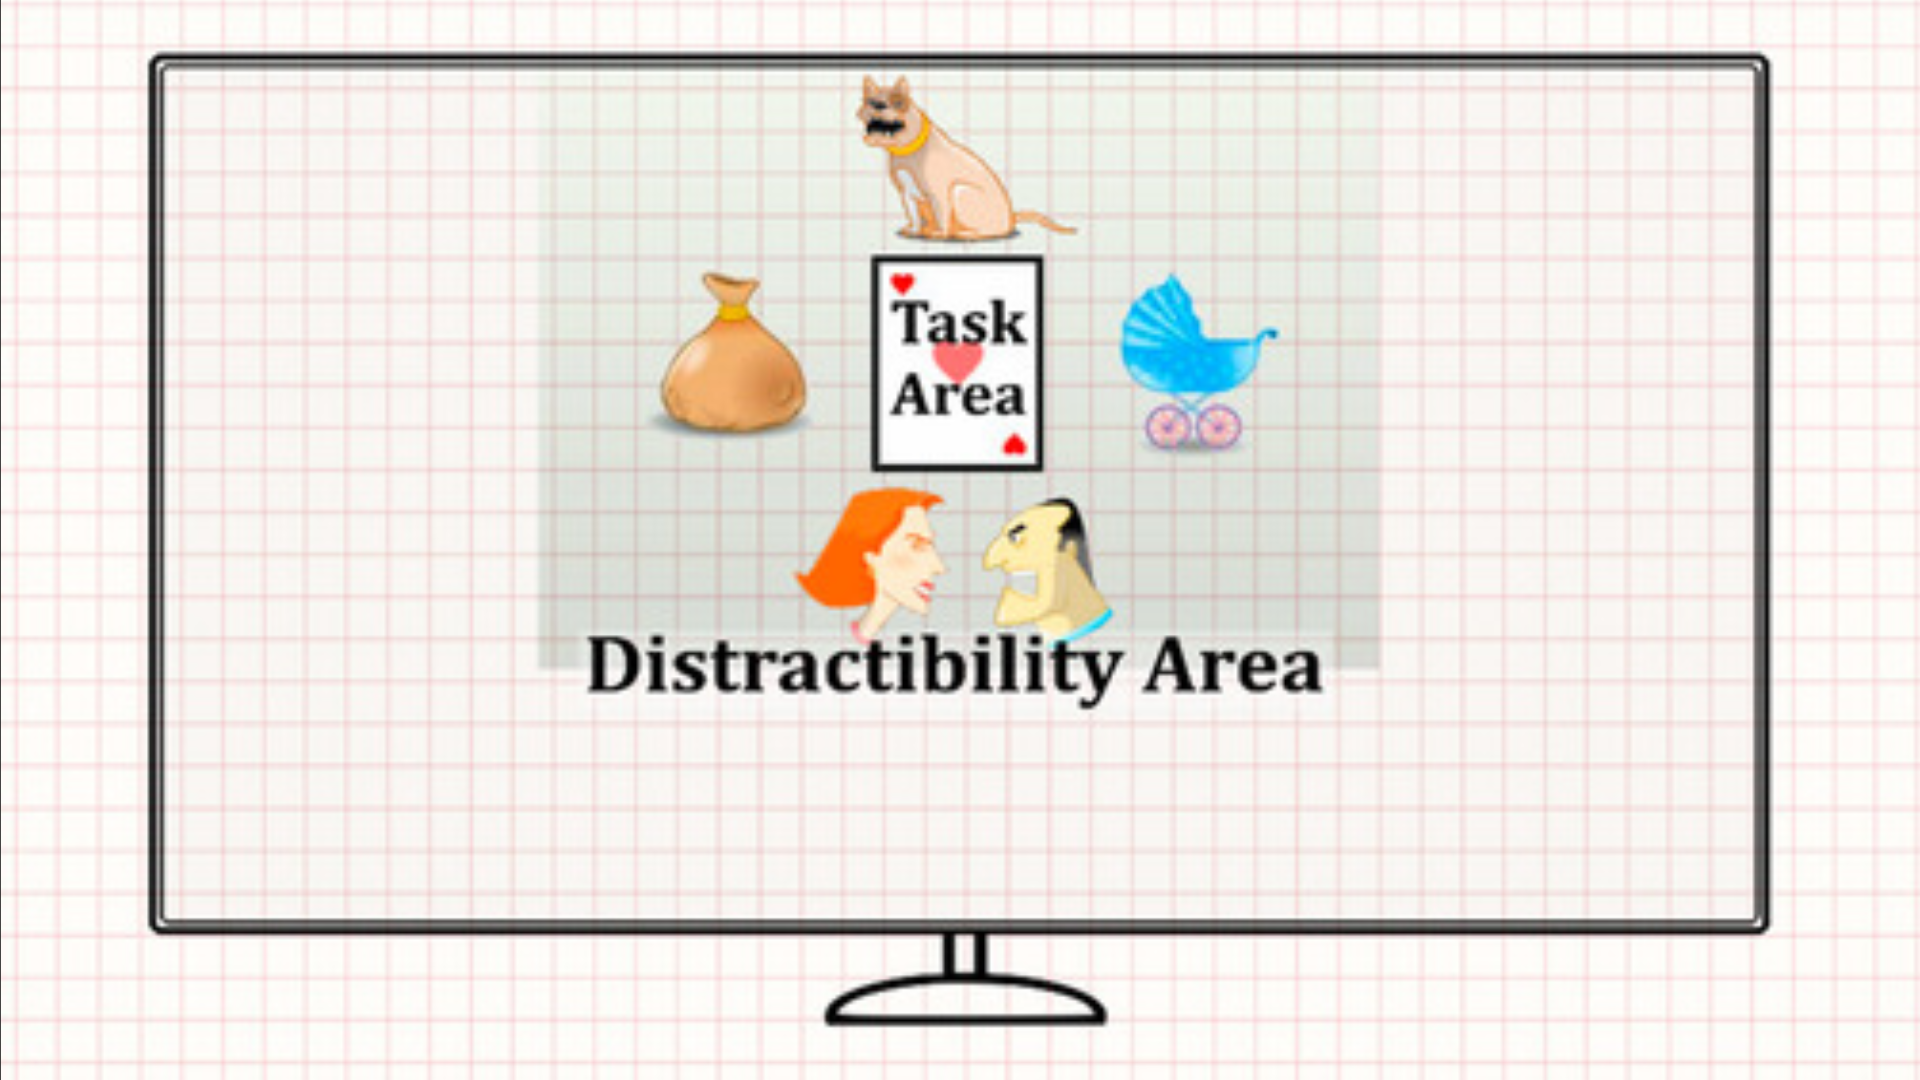
\includegraphics[width=\textwidth]{figuras/elb2020.png}
        
        \vspace{0.4cm}
        \textbf{Elbaum et al. (2020)}\\
        {\small
        Attention-Deficit/Hyperactivity Disorder (ADHD): Integrating the MOXO-dCPT with an Eye Tracker Enhances Diagnostic Precision
        }
    \end{column}

    \begin{column}{0.04\textwidth}
        \rule{0.5pt}{0.75\textheight}
    \end{column}

    \begin{column}{0.48\textwidth}
        \centering
        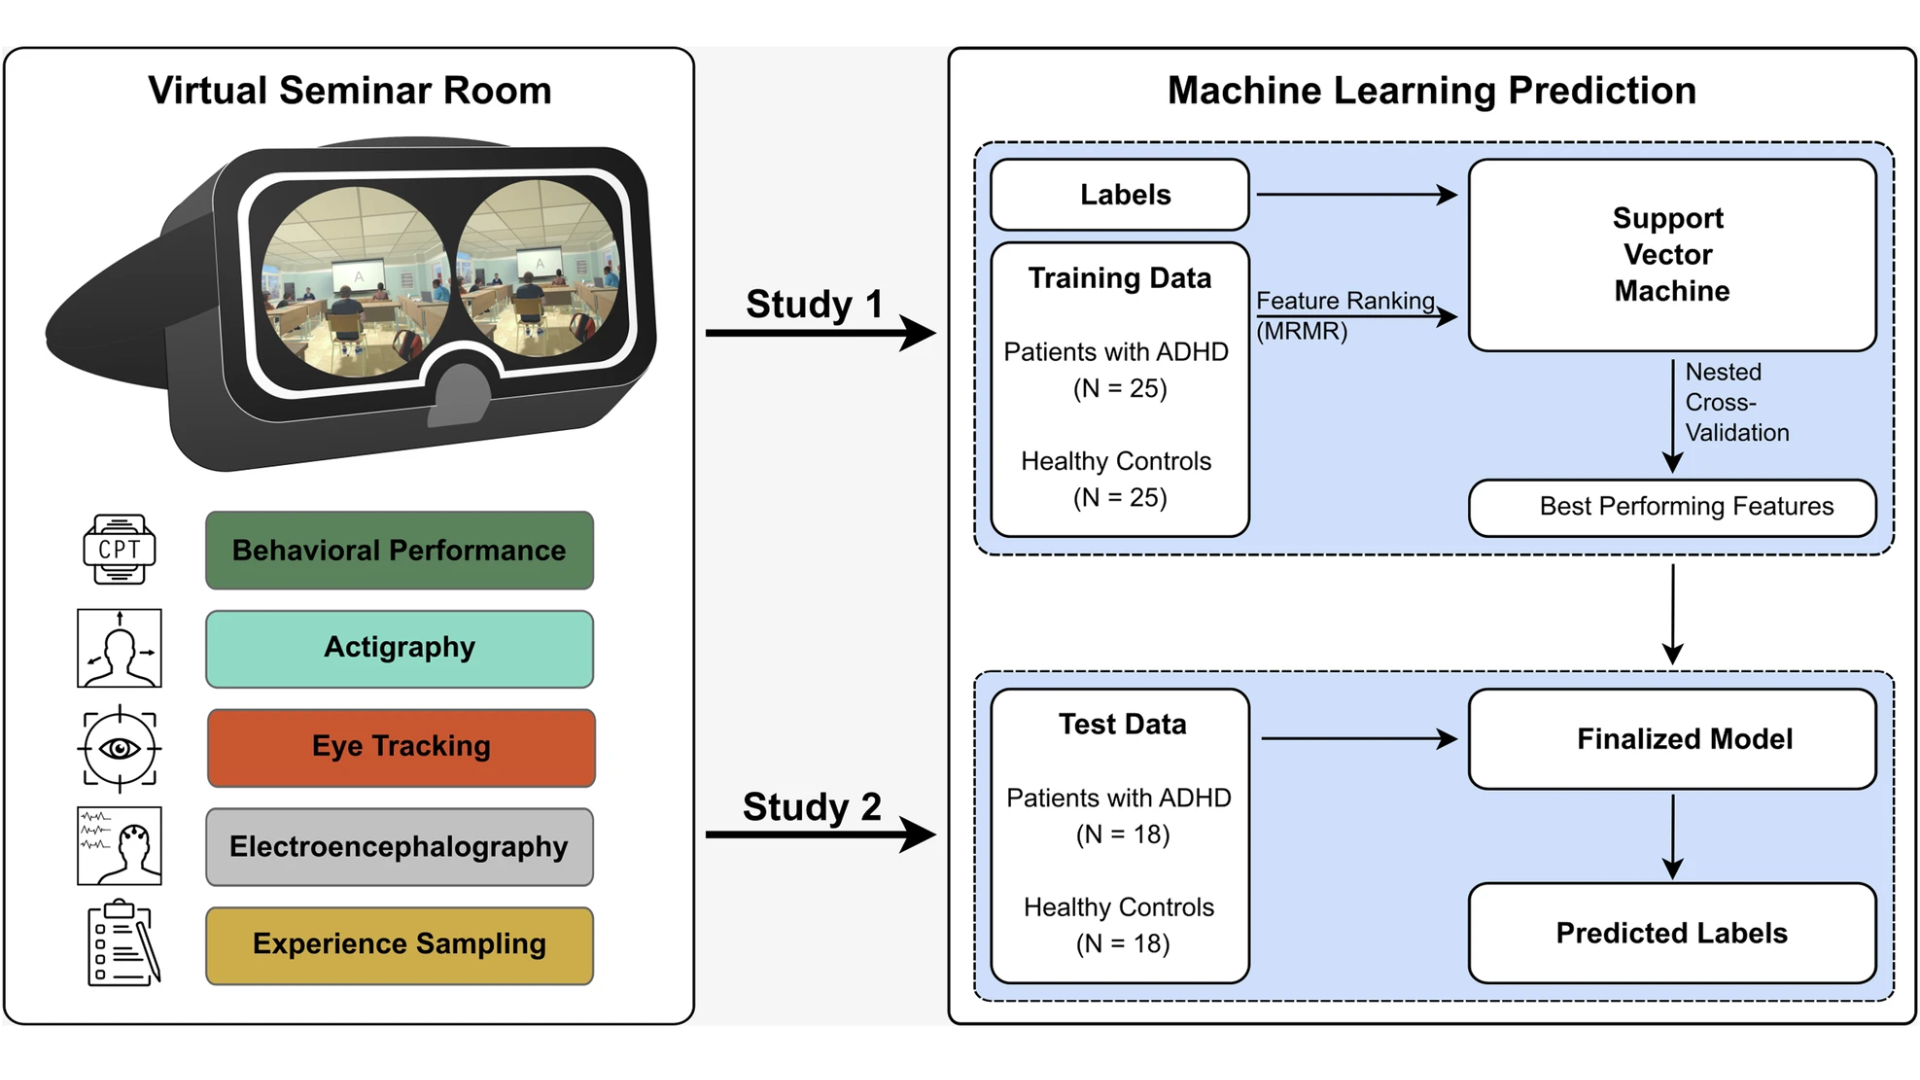
\includegraphics[width=\textwidth]{figuras/wie2024.png}

        \vspace{0.4cm}
        \textbf{Wiebe et al. (2024)}\\
        {\small
        Virtual reality-assisted prediction of adult ADHD based on eye tracking, EEG, actigraphy and behavioral indices: a machine learning analysis of independent training and test samples
        }
    \end{column}

\end{columns}

\end{frame}

\section{Objetivo}
\begin{frame}{Objetivo}
\justifying
\begin{enumerate}
  \item Integrar o TDC a um jogo digital com tarefas que
  simulam desafios atencionais.
  \item  Aplicar técnicas de \textit{eye tracking} em tempo real para registrar padrões de
  atenção durante a execução das tarefas.
  \item Processar automaticamente os dados coletados e compará-los com parâmetros
  normativos para gerar feedback ao usuário.
  \item Promover uma solução acessível, autônoma e alinhada ao ODS 3 da ONU, que amplie
  o acesso à triagem inicial de TDA.
\end{enumerate}
\end{frame}

\section{Metodologia}

% SLIDE 1
\begin{frame}{Metodologia — Parte 1}
\justifying

\begin{itemize}
    \item Adaptação do Teste de Desempenho Contínuo (TDC) para um jogo digital.
    \item Estrutura em três fases, com dificuldade progressiva.
    \item Coleta simultânea do desempenho (acertos, erros, tempo de resposta).
    \item Rastreamento ocular em tempo real durante todo o teste.
    \item Registro de padrões de foco e dispersão visual.
    % TODO: adicionar figura ilustrativa do jogo
\end{itemize}

\end{frame}

% SLIDE 2
\begin{frame}{Metodologia — Parte 2}
\justifying

\begin{itemize}
    \item Fases avaliam diferentes tipos de atenção:
    \begin{itemize}
        \item Sustentada
        \item Seletiva
        \item Alternada
        \item Dividida
    \end{itemize}
    \item Inserção de estímulos distratores visuais e sonoros.
    \item Ao final de cada fase, o sistema exibe o desempenho.
    \item No fim do teste, o sistema gera um indicador preliminar de atenção.
    % TODO: adicionar figura ilustrativa do jogo
\end{itemize}

\end{frame}

\section{Apresentação prática}
\begin{frame}{Apresentação prática}
\justifying
Mistura de etapas, ferramentas e resultados.  
Falta de clareza sobre o fluxo de desenvolvimento, separação entre metodologia de pesquisa e de implementação, e presença de trechos do modelo sem conteúdo autoral.
\end{frame}

\section{Resultados}
\begin{frame}{Resultados}
\justifying
Figuras muito pequenas ou sem legenda.  
Ausência de fluxogramas obrigatórios.  
Tabelas e seções de exemplo do modelo não substituídas adequadamente.
\end{frame}

\end{document}
